%! Author = UserHome
%! Date = 02.12.2024


\chapter{Heuristické algoritmy}

Táto kapitola sa zameriava na algoritmy, ktoré využívajú heuristické metódy na hľadanie riešení. Tieto algoritmy sú navrhnuté tak, aby rýchlo našli riešenie, aj keď nemusia zaručiť nájdenie optimálneho výsledku. Príkladmi sú algoritmy ako min-max konflikt a hill climbing, ktoré sa opierajú o lokálne úpravy aktuálneho stavu šachovnice.

\section*{Min-max konflikt}
File: solver/min-max-conflict.py\par

Najprv sa dámy umiestnia na šachovnicu do náhodných pozícií z domény ako je znázornené na obrázku \ref{fig:min-max-zero-step}.

Tento krok sa začína náhodným výberom kráľovnej s aspoň 1 konfliktom. Potom sa presunie na pozíciu v doméne, kde má najmenej konfliktov. Tento krok je znázornený na obrázku \ref{fig:min-max-step}. Tieto kroky sa vykonávajú, kým sa nenájde riešenie alebo kým sa nevyčerpá limit krokov.
\begin{figure}[h]
  \centering
  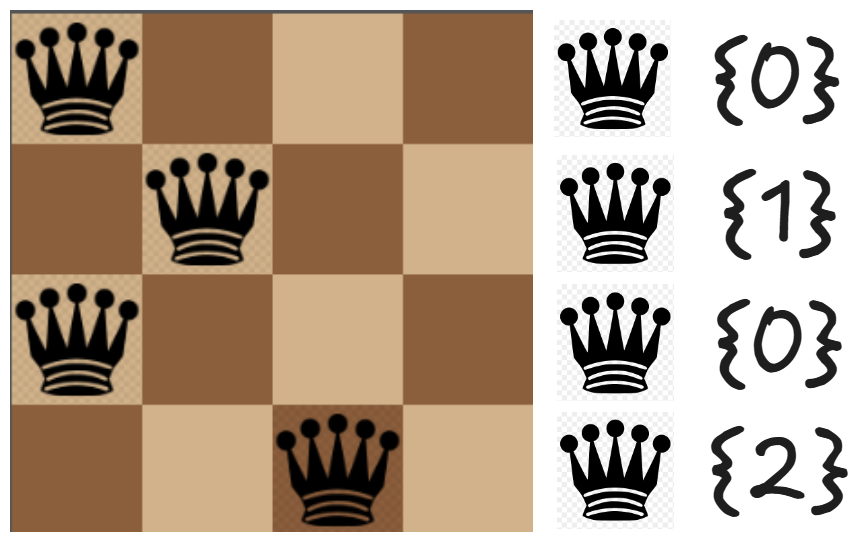
\includegraphics[width=0.6\textwidth]{figs/min-max/min-max-zero-step}
  \caption{Počiatočný stav pri min-max konflikte}
  \label{fig:min-max-zero-step}
\end{figure}
\begin{figure}[!h]
  \centering
  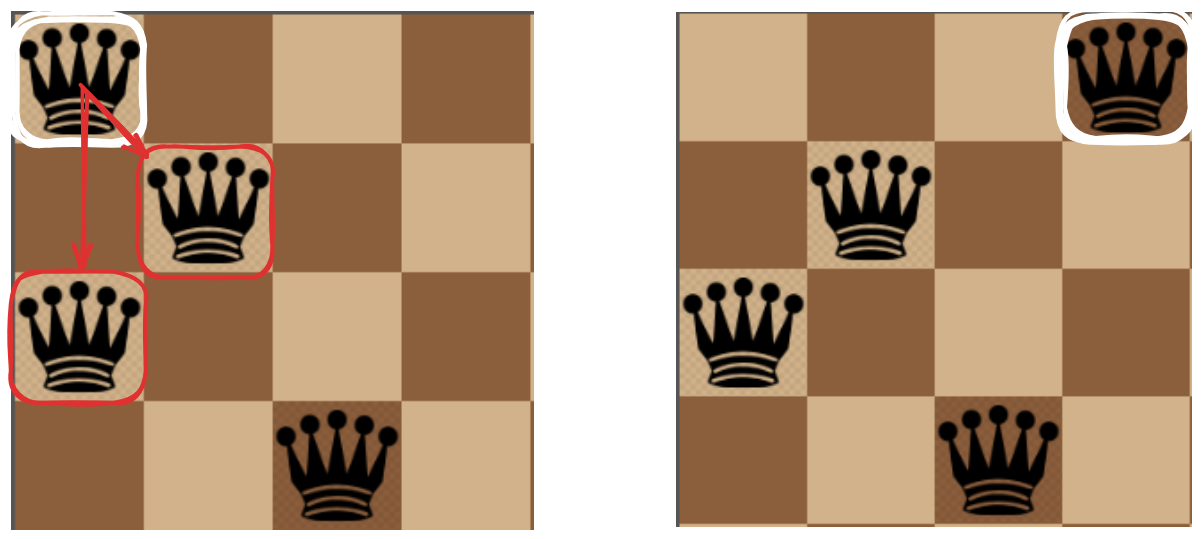
\includegraphics[width=0.8\textwidth]{figs/min-max/min-max-step}
  \caption{Presun dámy na pozíciu s najmenším počtom konfliktov pri min-max konflikte}
  \label{fig:min-max-step}
\end{figure}


\begin{table}[ht]
  \centering
  \begin{tabular}{|c|c|c|c|c|}
    \hline
    \textbf{Problem size} & \textbf{Avg Time Sec} & \textbf{Avg Nodes expanded} & \textbf{Limit moves} & \textbf{Success rate} \\
    \hline
    16                    & 0.007062385082        & 10                          & 10                   & 0.00\%                \\
    16                    & 0.04729111433         & 67                          & 100                  & 68.00\%               \\
    16                    & 0.05764730453         & 80.17                       & 1000                 & 100.00\%              \\
    \hline
    8                     & 0.002138266563        & 9.55                        & 10                   & 14.00\%               \\
    8                     & 0.00928393364         & 48.62                       & 100                  & 79.00\%               \\
    8                     & 0.01833538294         & 96.28                       & 1000                 & 95.00\%               \\
    \hline
    4                     & 0.000581178665        & 6.96                        & 10                   & 63.00\%               \\
    4                     & 0.000760693550        & 10.22                       & 100                  & 100.00\%              \\
    4                     & 0.000553886890        & 10                          & 1000                 & 100.00\%              \\
    \hline
  \end{tabular}
  \caption{Výsledky min-max conflict}\label{tab:table}
\end{table}




\section*{HillClimbing}

Algoritmus Hill Climbing je príkladom lokálneho vyhľadávania. Algoritmy tohto typu začínajú riešenie náhodným priradením hodnôt domény premenným a postupne sa snažia priviesť problém do konzistentného stavu.
Hill-climbing je greedy algoritmus, ktorý v každom kroku porovnáva všetky stavy, do ktorých sa môže dostať, s aktuálnym stavom a vyberá ten najlepší (bez ohľadu na buduce moznosti rozvoja tohto stavu). Na vyhodnotenie používa určitú funkciu (heuristiku), v našom prípade heuristickou funkciou je počet dvojíc kráľovien, ktoré na seba útočia.

Existujú aj modifikácie tohto algoritmu.

\begin{itemize}
  \item \textbf{Sideway moves:} Po vstupe do lokálneho minima sa algoritmus pokúsi vyjsť von, prechodom do susediacich stavov s rovnakou hodnotou heuristiky.
  \item \textbf{Random restart:} Algoritmus sa spustí niekoľkokrát v nádeji, že počiatočné usporiadanie kráľovien bude úspešnejšie.
\end{itemize}


Vďaka tejto metóde výberu ďalšieho stavu sa dosiahne neuveriteľne malý počet krokov, v priemere 4 kroky pre problém veľkosti 8. To je však kompenzované veľmi nízkou výkonnosťou algoritmu, keďže rieši približne 13 % usporiadaní kráľovien.  Táto situácia vzniká v dôsledku tendencie algoritmu uviaznuť v lokálnych minimách alebo „ramenách“. Ide o body, v ktorých heuristické hodnoty všetkých susedných stavov nie sú vyššie ako náš aktuálny stav, a preto algoritmus nemusí pokračovať v hľadaní.

Výsledky algoritmu sa dajú výrazne zlepšiť povolením pohybov do stavov s rovnakým skóre, ako má náš stav (Sideways moves).
Výsledky sú uvedené nižšie (bolo vykonané 100 spustení).
\begin{table}[ht]
  \centering
  \begin{tabular}{|c|c|c|c|c|}
    \hline
    \textbf{Problem size} & \textbf{Avg Time Sec} & \textbf{Avg Nodes expanded} & \textbf{Side moves} & \textbf{Success rate} \\
    \hline
    16                    & 0.01614097595         & 6.49                        & 0                   & 3.00\%                \\
    16                    & 0.06838754177         & 30.78                       & 50                  & 82.00\%               \\
    16                    & 0.07235177994         & 33.19                       & 100                 & 95.00\%               \\
    \hline
    8                     & 0.00145539999         & 3.09                        & 0                   & 13.00\%               \\
    8                     & 0.006260027885        & 17.8                        & 50                  & 92.00\%               \\
    8                     & 0.008184123039        & 23.68                       & 100                 & 94.00\%               \\
    \hline
    4                     & 0.0002376747131       & 1.56                        & 0                   & 37.00\%               \\
    4                     & 0.000291030407        & 3.02                        & 50                  & 100.00\%              \\
    4                     & 0.0001915192604       & 2.96                        & 100                 & 100.00\%              \\
    \hline
  \end{tabular}
  \caption{Výsledky hill climbing}\label{tab:table2}
\end{table}


\section{Zhrnutie}

Algoritmy pracujú veľmi podobne a zaberajú takmer rovnaký čas. Hill climbing sa však správa oveľa lepšie z hľadiska navštívených uzlov. Pri nízkych obmedzeniach (side moves alebo limit moves) obidva algoritmy takmer nikdy nenájdu výsledok, ale pri normálnych hodnotách sa výsledok našiel vo viac ako 90 \% prípadov.
